\newpage
\section{Theoretische Grundlagen}

\subsection{Zielsetzung}

\noindent
In diesem Versuch soll der Compton-Effekt untersucht werden. 
Dabei wird ein Plexiglaquader genutzt, der mit Röntgenstrahlung bestrahlt wird und dessen Transmissionsverhalten dann untersucht wird.

\subsection{Compton-Effekt}

\noindent
Der Compton-Effekt ist eine Wirkung, welche Auftritt wenn ein hochenergetisches Photon auf ein Elektron trifft. 
Das Photon wechselwirkt dabei mit dem Elektron, wobei es selbst Energie an das Elektron abgibt.

\begin{wrapfigure}{r}{6cm}[
    \centering
    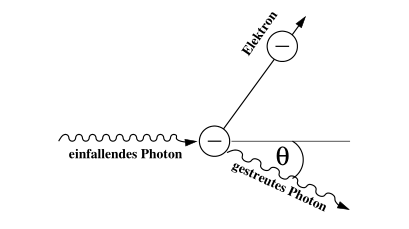
\includegraphics[width=6cm]{latex/images/Compton.PNG}
    \caption{Eine schematische Darstellung der Streuung eines Photons an einem Elektron\protect \cite{354}.}
    \label{img:comp}
\end{wrapfigure}

\noindent
Dadurch befindet sich das Elektron nun in Bewegung und das Photon besitzt eine längere Wellenlänge.\\
Da dieser Vorgang mit einem elastischem Stoß vergleichbar ist muss hier neben der Energie auch der Impuls erhalten bleiben.
Aus diesem Grund wird das Photon am Elektron gestreut um den Winkel $\theta$.\\
Zur grafischen Veranschaulichung des Vorgangs dient dabei Abbildung \ref{img:comp}\\
Die Wellenlänge des gestreuten Elektrons lässt sich dabei über die folgende Relation bestimmen:
\begin{equation*}
    \lambda_2-\lambda_1=\frac{\symup{h}}{\symup{m_e\cdot c}}\left(1-\cos(\theta)\right)
\end{equation*}
Dabei sind $\lambda_1$, $\lambda_2$ einfallende und ausfallende Wellenlänge, ${\symup{h}}$ das Planck'sche Wirkungsquantum\cite{Planck},
$\symup{m_e}$ die Ruhemasse des Elektrons\cite{me} und $\symup{ c}$ die Lichtgeschwindigkeit\cite{c}.\\
$\frac{\symup{h}}{\symup{m_e\cdot c}}$ wird dabei zusätzlich Compton-Wellenlänge $\lambda_C$ gennannt, 
da bei maximaler Wellenlängenverschiebung mit $\theta=\pi$, 
Der maximale Energieübertrag und damit die maximale Wellenlängenverschiebung findet bei $\theta=\pi$ statt. 
Dabei gilt $\lambda_2=2\cdot \lambda_C$ mit $\lambda_C=\frac{\symup{h}}{\symup{m_e\cdot c}}$ als Comptonwellenlänge.\\
Keine Energieübertragung findet bei $\theta=0$ statt.\\\\


\subsection{Röntgenstrahlung}

Um Röntgenstrahlung für die Untersuchung zu erzeugen werden in einer Röntgenröhre durch Glühemission freigewordene Elektronen auf eine Anode beschleunigt.\\
Dabei wird von der Anode ein kontinuirliches Spektrum an Bremsstrahlung und ein Anodenmaterial spezifisches, charakteristisches Röntgenspektrum emitiert.\\
Das kontinuirliche Bremsspektrum rührt daher, dass das auftreffende Elektron im Material von den Elektronen gebremst wird, wobei es seine Energie abstrahlt.
Diese abgestrahlte Energie hat dabei aber keine diskreten Werte wodurch das Spektrum kontinuirlich wird.\\
Das charakteristische Röntgenspektrum kommt von im Metall durch Stoßprozesse angeregt, gebundene Elektronen, die anschließend für diskrete Energien Röntgenstrahlung abstrahlen.\\\\

\noindent
Zur Untersuchung der Comptonwellenlänge wird das Transmissionsverhalten von Aluminium genutzt. 
Da die Absorption von Licht mit zunehmender Wellenlänge abnimmt, lässt sich durch einen Vergleich der Intensität des ungebeugten Lichts mit der des gebeugten Lichts, Rückschlüsse über dessen Wellenlänge schließen.\\
Dafür wird dann diese Gleichung genutzt, die eine Relation zwischen der Intensität des einfallenden Lichts $I_0$ und der des abgeschwächten austretenden $I$, herstellt:
\begin{equation*}
    I= I_0\cdot \symup{e}^{-\mu\cdot d}
\end{equation*}
$d$ ist dabei die Dicke des Materials und $\mu$ der Absorptionskoeffizient, welcher sich aus den Absorptionskoeffizienten für Paarbildung $\mu_{Paar}$, für den Photoeffekt $\mu_{Photo}$
und für den Comptoneffekt $\mu_{Compton}$, summiert zusammensetzt.\\\\

\noindent Die Energie  der Photonen lässt sich mit Hilfe der Bragg'schen-Reflexion bestimmen.

\begin{wrapfigure}{r}{5cm}[
    \centering
    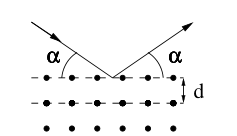
\includegraphics[width=5cm]{latex/images/Bragg.PNG}
    \caption{Eine schematische Darstellung der Reflexion eines Photons an polykristalliner Materie\protect \cite{V354}.}
    \label{img:bragg}
\end{wrapfigure}

\noindent
Dabei bestrahlt man ein Gitter unter dem Winkel $\alpha$ mit Röntgenstrahlung.
Bei richtiger Wahl des Glanzwinkels $\alpha$ wird das Licht so reflektiert und gebrochen, dass es mit dem von der unterliegenden Gitterebene reflektierten und gebrochendm Licht konstruktiv interferiert.\\
Schematisch dargestellt ist dieser Vorgang in der nebenstehenden Abbildung \ref{img:bragg}.\\
Die richtige Wahl des Winkels erfüllt dabei folgende Wellenlängenabhängigkeit:
\begin{equation*}
    2d \cdot \sin(\alpha)=n\cdot \lambda
    \label{eqn:bragg}
\end{equation*}
Dabei ist $d$ die Entfernung der Gitterebenen und $n$ die Beugungsordnung des Lichts.


